%% ============================================================
%% NSF CMMT / CDS&E Proposal
%% QMatBridge: Reproducible Benchmark Infrastructure for
%% First-Quantized Hamiltonian Simulation of Materials
%%
%% PI: Roberto dos Reis
%%     Research Assistant Professor
%%     Department of Materials Science and Engineering
%%     Northwestern University
%%
%% Program: NSF DMR -- Condensed Matter and Materials Theory (CMMT)
%%          via Computational and Data-Enabled Science and Engineering
%%          (CDS&E) submission route (NSF 23-611)
%%
%% Formatting: NSF PAPPG compliant
%%   - 8.5 x 11 in, 1-inch margins
%%   - 11pt Palatino (allowed font per PAPPG)
%%   - No page limit on References Cited section
%%   - Project Description: 15 pages
%% ============================================================

\documentclass[11pt]{article}

\usepackage[margin=1in]{geometry}
\usepackage[T1]{fontenc}
\usepackage{palatino}           % NSF-allowed 11pt font
\usepackage{microtype}
\usepackage{setspace}
\usepackage{parskip}
\usepackage{titlesec}
\usepackage{enumitem}
\usepackage{booktabs}
\usepackage{array}
\usepackage{tabularx}
\usepackage{multirow}
\usepackage{xcolor}
\usepackage{mdframed}
\usepackage{amsmath, amssymb}
\usepackage{graphicx}
\usepackage{url}
\graphicspath{{./}}
\usepackage[colorlinks=true, linkcolor=blue!70!black,
            citecolor=blue!70!black, urlcolor=blue!70!black]{hyperref}
\usepackage[numbers, sort&compress]{natbib}
\usepackage{fancyhdr}
\usepackage{lastpage}

%% --- Typography ---
\setlength{\parindent}{0pt}
\setlength{\parskip}{5pt plus 1pt}
\setstretch{1.05}

%% --- Section headings ---
\definecolor{nsfblue}{RGB}{30,70,130}
\titleformat{\section}{\large\bfseries\color{nsfblue}}{}{0em}{}[\titlerule]
\titleformat{\subsection}{\normalsize\bfseries}{}{0em}{}
\titleformat{\subsubsection}{\normalsize\itshape}{}{0em}{}
\titlespacing{\section}{0pt}{10pt}{4pt}
\titlespacing{\subsection}{0pt}{7pt}{2pt}

%% --- Header / footer ---
\pagestyle{fancy}
\fancyhf{}
\renewcommand{\headrulewidth}{0.4pt}
\fancyhead[L]{\small\textit{QMatBridge --- NSF CMMT/CDS\&E --- Dos Reis, Northwestern MSE}}
\fancyhead[R]{\small\thepage}
\fancyfoot{}

%% --- Framed boxes ---
\mdfdefinestyle{aimbox}{
  linecolor=nsfblue, linewidth=1.2pt,
  backgroundcolor=blue!4,
  innerleftmargin=8pt, innerrightmargin=8pt,
  innertopmargin=6pt, innerbottommargin=6pt,
  skipabove=6pt, skipbelow=6pt
}

%% --- Math shorthands ---
\newcommand{\la}{\lambda}
\newcommand{\de}{\delta\varepsilon}
\newcommand{\Ecut}{E_{\mathrm{cut}}{}}
\newcommand{\nb}{{n_b}}
\newcommand{\NPW}{N_{\mathrm{PW}}}
\newcommand{\tgate}{\widetilde{T}}
\newcommand{\qprox}{q_{\mathrm{prox}}}
\newcommand{\score}{\mathcal{S}}

%% ============================================================
\begin{document}

%% ============================================================
\thispagestyle{empty}
\begin{center}
  {\LARGE\bfseries\color{nsfblue} Project Summary}\\[6pt]
  {\large QMatBridge: Open Cyberinfrastructure for Reproducible\\
  First-Quantized Hamiltonian Simulation Benchmarks}\\[4pt]
  {\normalsize
  Roberto dos Reis $\cdot$ Department of Materials Science and Engineering
  $\cdot$ Northwestern University\\
  NSF DMR -- CMMT (CDS\&E route) $\cdot$ NSF 23-611}
\end{center}

\noindent\rule{\linewidth}{0.6pt}

\subsection*{Overview}

Research groups developing fault-tolerant Hamiltonian simulation algorithms
--- block-encodings, qubitization circuits, linear-combination-of-unitaries
(LCU) decompositions --- require realistic electronic-structure Hamiltonians
to test and benchmark their primitives against physically meaningful targets.
The standard path today is a collection of private, incompatible scripts that
pull density functional theory (DFT) data from databases such as the
Materials Project~\cite{Jain2013} or OQMD~\cite{Kirklin2015}, reformat the
data, and feed it into a quantum compiler.
These scripts are almost never shared, rarely interoperable with more than one
quantum framework, and frequently omit the provenance information required to
reproduce or compare results across institutions.
When two groups report T-gate counts for the same material, there is no
current mechanism to verify they used the same Hamiltonian, the same
basis-set parameters, or the same LCU decomposition conventions.

\textbf{QMatBridge} addresses this structural gap by providing an open-source,
dependency-free neutral intermediate representation (NIR) that any upstream
database adapter can write to and any downstream quantum resource estimator
or compiler can read from, with full provenance embedded at the record level.
This proposal requests support to (i)~complete the QMatBridge v0.2--v0.5
development roadmap, including live Materials Project and OPTIMADE adapters;
(ii)~build and curate a Tier-1 benchmark fixture set spanning five
representative crystalline materials; (iii)~implement exporters for
OpenFermion~\cite{McClean2020}, Qualtran~\cite{Qualtran2023}, and
pyLIQTR~\cite{pyLIQTR2023}; and (iv)~establish a community benchmark
standard through open governance and a dedicated sensitivity-analysis
framework for resource-estimate parameter studies.

\subsection*{Intellectual Merit}

The proposed work advances the computational and data-centric methodology of
materials research in three ways.
First, a \emph{canonical hash} (SHA-256 over physically meaningful fields of
a \texttt{QMatEntry} record) provides a unique, database-independent identity
for each Hamiltonian, enabling benchmark reproducibility at the record level
and directly addressing the cross-code reproducibility crisis documented in
DFT~\cite{Lejaeghere2016}.
Second, a \emph{reproducible sensitivity analysis framework} --- demonstrated
in preliminary results --- identifies which input controls (plane-wave cutoff
energy, energy precision target $\de$, and orbital band count $\nb$) govern
estimated T-gate and qubit resource costs; the analysis reveals that $\de$
dominates with near-unit inverse elasticity ($\varepsilon \approx -1.01$),
providing a quantitative planning heuristic with direct implications for
benchmark selection and hardware targeting.
Third, the QMatBridge \emph{oracle metadata layer} stores LCU 1-norms,
SELECT/PREPARE circuit parameters, and complexity annotations in a
structured, queryable format, enabling systematic multi-material Pareto
analysis across competing resource objectives and supporting the
algorithm--materials co-design cycle.

\subsection*{Broader Impacts}

QMatBridge directly addresses a community infrastructure deficit affecting
every research group at the interface of computational materials science and
fault-tolerant quantum algorithms.
All outputs are MIT-licensed with an open governance model.
Situated at Northwestern University's MSE department --- with existing
connections to the Argonne National Laboratory quantum computing program and
the NSF-funded Institute for Quantum Information Research and Engineering
(INQUIRE) at Northwestern --- the project bridges the DFT computation
community and the quantum algorithms community, providing training
opportunities for graduate students at this increasingly demanded interface.
The benchmark suite is designed for integration into graduate courses on
quantum algorithms and materials informatics, and the CDS\&E submission
route reflects the project's explicit commitment to software sharing,
FAIR data principles~\cite{Wilkinson2016}, and long-term community
maintainability.

\newpage
\setcounter{page}{1}

%% ============================================================
\begin{center}
  {\LARGE\bfseries\color{nsfblue} Project Description}\\[4pt]
  {\large QMatBridge: Open Cyberinfrastructure for Reproducible\\
  First-Quantized Hamiltonian Simulation Benchmarks}
\end{center}
\noindent\rule{\linewidth}{0.6pt}

%% ============================================================
\section{Introduction and Motivation}

Fault-tolerant quantum simulation of electronic structure holds the
potential to resolve long-standing challenges in materials science ---
including the accurate treatment of strongly correlated electron systems,
prediction of high-temperature superconductors, and design of transition-metal
catalysts --- that remain intractable for classical computation at the
required accuracy~\cite{Reiher2017,vonBurg2021,Goings2022}.
The theoretical framework for these simulations is now mature: first-quantized
plane-wave Hamiltonians combined with qubitization or LCU decompositions
provide asymptotically optimal fault-tolerant algorithms for periodic
materials~\cite{Babbush2019,Su2021,Lee2021}, with well-characterized
T-gate and qubit resource estimates scaling as $\mathcal{O}(\lambda/\de)$
and $\mathcal{O}(\log N_{\mathrm{PW}})$, respectively, where $\lambda$ is
the LCU 1-norm, $\de$ is the target energy precision, and
$N_{\mathrm{PW}}$ is the number of plane-wave basis functions.

Despite this theoretical maturity, the field lacks a shared data
infrastructure connecting classical DFT databases to these quantum algorithms.
A researcher wishing to benchmark a new LCU circuit variant against bulk
silicon must currently: (1)~access the Materials Project API~\cite{Jain2013}
and extract structure, basis-set parameters, and pseudopotential metadata;
(2)~reformat this data into the conventions of a specific quantum compiler;
(3)~compute the LCU 1-norm $\lambda$ according to the conventions of their
chosen decomposition; and (4)~record sufficient metadata for others to
reproduce the computation.
Each step is currently performed with private, group-specific scripts that
are incompatible across groups.
The consequence, documented in analogy with the DFT reproducibility
crisis~\cite{Lejaeghere2016}, is that T-gate estimates for the same physical
system vary substantially across publications --- not due to algorithmic
differences but due to inconsistent Hamiltonian parameterization.

\textbf{QMatBridge} resolves this by providing an open-source, zero-dependency
neutral intermediate representation (NIR) for first-quantized electronic
Hamiltonians.
The framework defines a \texttt{QMatEntry} schema that records the full
provenance chain from upstream database to oracle metadata, exposes a
deterministic canonical hash for record identity, and is designed to be
targeted by any database adapter and consumed by any quantum compiler or
resource estimator.
This proposal requests CDS\&E support to complete the adapter and exporter
layers, build a Tier-1 community benchmark fixture set, and establish the
sensitivity analysis framework as a reproducible methodology for parameter
studies in quantum simulation planning.

\textbf{New science enabled.}
QMatBridge is not a convenience tool; it makes scientifically distinct
studies possible.
Three classes of investigation that are currently impossible without it:
(1)~\emph{Cross-group $\lambda$ reproducibility studies}: by providing a
canonical hash, two independent groups can verify for the first time that
their T-gate estimates are based on the same Hamiltonian, enabling the first
systematic meta-analysis of resource estimation uncertainty across the
literature.
(2)~\emph{Precision-target optimization}: the sensitivity analysis framework
allows systematic identification of the $\de$ threshold below which
resource costs increase super-linearly for each material class, informing
hardware roadmap targeting in a way not previously quantified.
(3)~\emph{Multi-functional consistency studies}: by supporting PBE,
PBEsol, HSE06, and r$^2$SCAN via the Alexandria adapter, QMatBridge enables
quantification of how functional choice shifts $\lambda$ for strongly
correlated materials, directly informing which materials require HSE06-level
accuracy for reliable resource estimates.

\textbf{Community validation of the gap.}
The need for reproducible quantum simulation benchmark infrastructure is
independently recognized across the field, though existing efforts address
adjacent rather than overlapping problem domains.
Clark et al.\ (NQAC, 2026)~\cite{Clark2026} are developing an open-source,
executable benchmark framework for \emph{near-term quantum chemistry algorithms
on molecular systems} (second-quantized, small molecules, NISQ hardware).
QREChem~\cite{QREChem2023} provides logical resource estimation for
\emph{molecular} ground-state energy calculations via Trotter-based QPE.
ArQTiC~\cite{ArQTiC2022} enables near-term simulation of \emph{materials
governed by one-dimensional Heisenberg Hamiltonians} (real- and imaginary-time
evolution, near-term hardware).
None of these tools addresses \emph{periodic crystalline solids} in the
\emph{first-quantized, fault-tolerant} regime --- the regime in which quantum
advantage over classical DFT is expected to emerge for industrially relevant
bulk materials~\cite{vonBurg2021,Yoshioka2022}.
QMatBridge is designed precisely for this unoccupied niche.
Rather than competing with Clark et al., QREChem, or ArQTiC, QMatBridge is the
\emph{materials-and-fault-tolerant counterpart} to these molecular and near-term
tools: the four together cover the full spectrum from small molecules on NISQ
hardware to periodic crystals on fault-tolerant hardware.

\begin{figure}[h!]
\centering
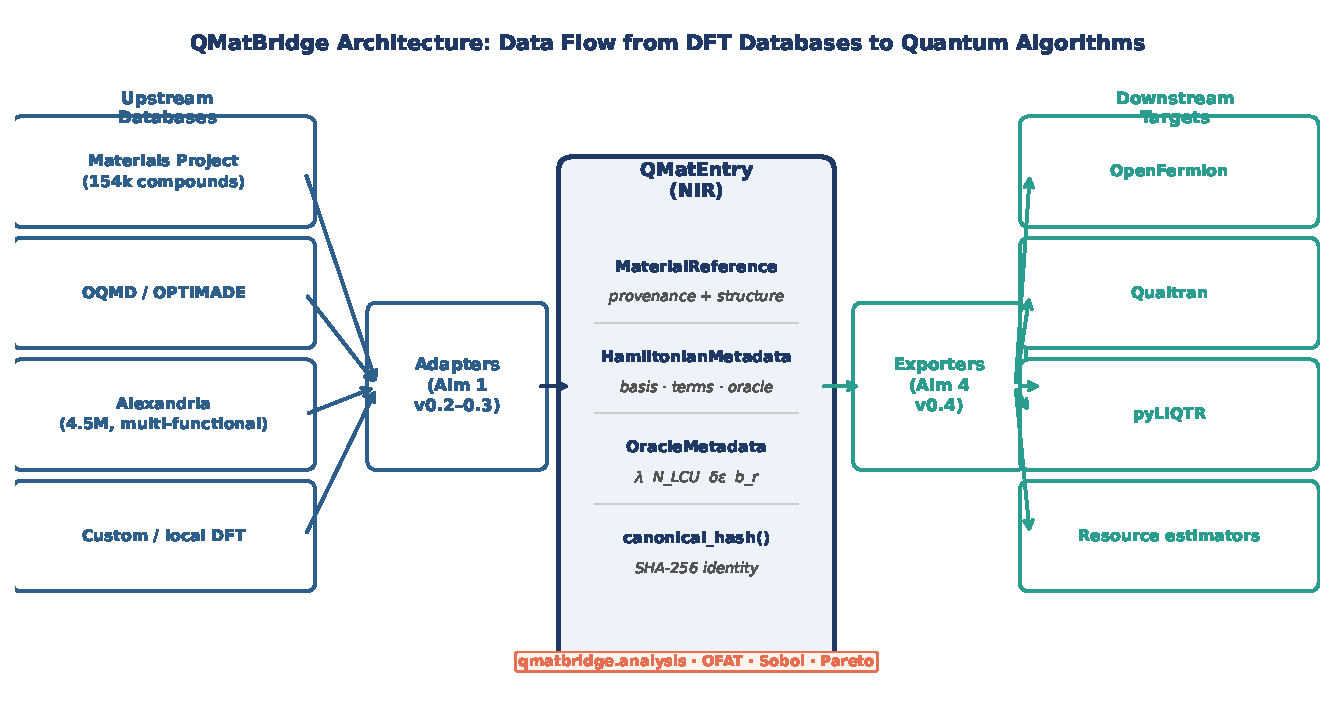
\includegraphics[width=\linewidth]{fig_architecture.pdf}
\caption{QMatBridge architecture. Adapters (Aim~1) translate upstream database
records into a versioned, hash-addressed \texttt{QMatEntry} neutral intermediate
representation (NIR). Exporters (Aim~4) translate the NIR into formats consumed
by downstream quantum compilers and resource estimators. The
\texttt{qmatbridge.analysis} module (Aim~3) operates on libraries of
\texttt{QMatEntry} records to produce sensitivity analyses and Pareto
frontier rankings. All components are dependency-free at the core schema level.}
\label{fig:arch}
\end{figure}

%% ============================================================
\section{Background}

\subsection{First-Quantized Hamiltonian Simulation}

In the first-quantized plane-wave formalism~\cite{Babbush2019,Su2021},
the electronic Hamiltonian of a periodic crystalline material is partitioned
as $H = T + U + V$, where $T$ is the kinetic energy operator (diagonal in
momentum space), $U$ is the electron--electron Coulomb interaction, and $V$
is the electron--nuclear interaction.
The LCU decomposition expresses $H = \sum_\ell \alpha_\ell H_\ell$, where
the $H_\ell$ are unitary operators and $\alpha_\ell \geq 0$ are real
coefficients.
The total LCU 1-norm $\lambda = \sum_\ell \alpha_\ell$ controls the dominant
cost of qubitized quantum phase estimation (QPE)~\cite{Low2019}:
the number of Toffoli gates scales as $\mathcal{O}(\lambda / \de)$,
where $\de$ is the target energy precision.
For bulk silicon at a 520~eV plane-wave cutoff, representative values are
$\lambda \approx 316$~Ha and $N_{\mathrm{PW}} \approx 1849$ plane waves
per spin channel, yielding a state register of $\lceil \log_2 N_{\mathrm{PW}}
\rceil = 11$ qubits~\cite{Babbush2019}.

This formalism is the basis for a growing body of material-specific resource
estimates~\cite{Reiher2017,vonBurg2021,Goings2022,Yoshioka2022},
but the underlying Hamiltonians are not shared, making cross-study comparison
unreliable.
The QMatBridge \texttt{OracleMetadata} schema is designed to store precisely
the quantities needed for reproducible qubitization resource estimation:
$\lambda$, $N_{\mathrm{LCU}}$, $\de$, $\eta$ (phase-error target),
$\lceil \log_2 N_{\mathrm{PW}} \rceil$, and the number of rotation bits
$b_r$, along with per-term breakdowns for $T$, $U$, and $V$.

\subsection{The Reproducibility Gap}

The materials DFT community confronted an analogous reproducibility crisis
in 2016, when Lejaeghere et al.~\cite{Lejaeghere2016} compared 40 DFT codes
computing equations of state for 71 elemental solids and found systematic
deviations attributable to basis-set conventions, pseudopotential families,
and code-specific defaults.
The resolution required not algorithmic innovation but infrastructure:
standardized input files, public reference data sets, and cross-code
validation workflows.

The quantum simulation community faces a structurally identical problem,
with added complexity: the connection between DFT outputs and quantum
algorithm inputs involves non-trivial transformations (plane-wave count
computation, LCU norm assembly, rotation-bit sizing) that are currently
performed differently in each group's codebase.
QMatBridge addresses this at the infrastructure level by defining the
transformation chain in a single, public, versioned schema and implementing
it in a reference codebase subject to continuous integration testing.

\subsection{Existing Software Landscape and Innovation Gap}

Table~\ref{tab:landscape} positions QMatBridge against the current
software ecosystem.
No existing tool simultaneously provides database-agnostic provenance
tracking, a canonical Hamiltonian identity, and direct export to
multiple fault-tolerant quantum compilers.

\begin{table}[h!]
\centering
\caption{Comparison of QMatBridge with existing software at the
DFT--quantum algorithm interface.
\checkmark = supported; \textemdash{} = not supported; $\sim$ = partial.}
\label{tab:landscape}
\small
\setlength{\tabcolsep}{5pt}
\begin{tabular}{lcccccc}
\toprule
Feature & OpenFermion & Qualtran & pyLIQTR & AiiDA & pymatgen & \textbf{QMatBridge}\\
\midrule
DFT database adapters       & \textemdash & \textemdash & \textemdash & $\sim$      & $\sim$      & \checkmark\\
Canonical Hamiltonian hash  & \textemdash & \textemdash & \textemdash & \textemdash & \textemdash & \checkmark\\
First-quantized LCU schema  & \textemdash & $\sim$      & $\sim$      & \textemdash & \textemdash & \checkmark\\
Multi-compiler export       & $\sim$      & \textemdash & \textemdash & \textemdash & \textemdash & \checkmark\\
Sensitivity / Pareto tools  & \textemdash & \textemdash & \textemdash & \textemdash & \textemdash & \checkmark\\
Zero-dependency core        & \checkmark  & \textemdash & \textemdash & \textemdash & \textemdash & \checkmark\\
Community benchmark fixtures& \textemdash & \textemdash & \textemdash & \textemdash & \textemdash & \checkmark\\
\midrule
\multicolumn{7}{l}{\textit{Scope comparison with adjacent near-term / molecular tools:}}\\
\midrule
Periodic cryst.\ (fault-tolerant) & \textemdash & $\sim$ & $\sim$ & \textemdash & \textemdash & \checkmark\\
Molecular (NISQ / near-term) & \checkmark & $\sim$ & $\sim$ & \textemdash & \textemdash & \textemdash\\
Provenance from DFT database & \textemdash & \textemdash & \textemdash & $\sim$ & $\sim$ & \checkmark\\
\bottomrule
\end{tabular}

\vspace{2pt}
{\footnotesize
\textit{Adjacent tools not shown above (different scope):}
ArQTiC~\cite{ArQTiC2022} (near-term, 1D Heisenberg materials);
QREChem~\cite{QREChem2023} (fault-tolerant resource estimation, molecular);
Clark et al.~\cite{Clark2026} (near-term benchmark framework, molecular).
None of the three targets periodic crystalline solids with first-quantized
fault-tolerant algorithms or DFT database provenance.}
\end{table}

QMatBridge's two most distinctive innovations are (i) the \emph{canonical
hash}, which for the first time gives fault-tolerant quantum simulation
benchmarks a database-independent, tamper-evident identity analogous to a DOI
for a specific Hamiltonian, and (ii) the \emph{sensitivity analysis framework},
which transforms resource estimation from a single-point calculation into a
reproducible parameter study, enabling systematic reasoning about where
quantum advantage thresholds are most sensitive to computational choices.

The adjacent tools ArQTiC~\cite{ArQTiC2022}, QREChem~\cite{QREChem2023},
and the recently funded Clark et al.\ benchmarking project~\cite{Clark2026}
address complementary but distinct problem spaces: near-term hardware,
second-quantized molecular Hamiltonians, or one-dimensional lattice models.
Their existence independently validates the community's recognition that
benchmark infrastructure is a field-wide need.
QMatBridge fills the remaining gap: \emph{periodic crystalline materials,
first-quantized plane-wave basis, fault-tolerant algorithms, and DFT database
provenance} --- the combination required for practical quantum advantage in
bulk materials simulation~\cite{vonBurg2021,Yoshioka2022,Beverland2022}.
None of the existing or adjacent tools is architecturally positioned to
fill this niche, because all of them begin after the Hamiltonian is already
specified and are not connected to the upstream DFT database ecosystem.

%% ============================================================
\section{Preliminary Results}

The QMatBridge v0.1 codebase~\cite{QMatBridge2026} demonstrates the
feasibility of the proposed approach across four independent dimensions.

\subsection{Schema and Canonical Hash (v0.1)}

The \texttt{QMatEntry} schema is implemented as a dependency-free Python
dataclass hierarchy comprising \texttt{MaterialReference} (provenance +
structure), \texttt{HamiltonianMetadata} (basis, terms, oracle), and
\texttt{OracleMetadata} (LCU decomposition parameters).
The \texttt{canonical\_hash()} method computes a SHA-256 digest over
12 physically meaningful fields (upstream source, functional, formula,
spacegroup, electron count, spin polarization, basis type, cutoff energy,
band count, and oracle precision target), providing a stable identity
that is invariant to metadata changes but sensitive to any physically
relevant modification.
A concrete silicon entry (mp-149, PBE/PAW\_PBE/VASP, 520~eV cutoff,
$\lambda = 315.8$~Ha, $\de = 10^{-3}$~Ha) has been implemented and
validated against the published resource estimates of Babbush et
al.~\cite{Babbush2019}, confirming that the schema captures all
quantities required to reproduce the literature estimate.

\subsection{Sensitivity Analysis of Resource Estimates}

A one-factor-at-a-time (OFAT) sensitivity analysis was performed over
three principal input controls of the silicon-like baseline:
$\Ecut \in \{400, 450, 500, 550, 600\}$~eV,
$\de \in \{5 \times 10^{-4}, 10^{-3}, 2 \times 10^{-3}\}$~Ha, and
$\nb \in \{12, 16, 20, 24\}$ bands.
Proxy models for the sweep are:
\begin{align}
  \NPW &= \NPW^{(0)}
         \!\left(\frac{\Ecut}{\Ecut^{(0)}}\right)^{\!3/2}, \quad
  n_{\mathrm{state}} = \lceil\log_2 \NPW\rceil, \quad
  n_{\mathrm{rot}} = \lceil{-\log_2 \de}\rceil + 10,
  \label{eq:qubits}\\
  \lambda &= \lambda^{(0)}
             \!\left(\frac{\Ecut}{\Ecut^{(0)}}\right)^{\!1/2}
             \!\left(\frac{\nb}{\nb^{(0)}}\right)^{\!1/4},
  \label{eq:lambda}\\
  \tgate &= \lambda / \de, \quad
  \qprox = n_{\mathrm{state}} + n_{\mathrm{rot}}, \quad
  \score = \tgate \!\left(1 + \qprox/100\right),
  \label{eq:score}
\end{align}
where superscript $(0)$ denotes baseline values
($\lambda^{(0)} = 315.8$~Ha, $\Ecut^{(0)} = 520$~eV,
$\NPW^{(0)} = 1849$, $\nb^{(0)} = 16$).
The formulas in Eqs.~\eqref{eq:qubits}--\eqref{eq:score} are explicit
planning proxies, not material-specific resource estimates: the $\lambda$
exponents (0.5 in $\Ecut$, 0.25 in $\nb$) are motivated by reciprocal-space
volume scaling arguments and should be replaced by computed values from the
Babbush et al.\ formula~\cite{Babbush2019} once the v0.2 adapter is live
(Aim~2). All exponents and constants are documented in the
output JSON metadata for independent verification.

The resulting tornado impact ranking (Table~\ref{tab:tornado}) reveals
that the energy precision target $\de$ is the dominant control by a
substantial margin, with 151.9\% relative impact and a local arc
elasticity $\varepsilon_\de \approx -1.01$ --- confirming near-unit
inverse proportionality between the composite resource score and $\de$.
The cutoff energy and band count exhibit sublinear effects, with
elasticities $\varepsilon_{E_{\mathrm{cut}}} \approx +0.50$ and
$\varepsilon_\nb \approx +0.25$, respectively, consistent with the
power-law exponents in Eq.~\eqref{eq:lambda}.

\begin{table}[h!]
\centering
\caption{Tornado impact summary from one-factor-at-a-time sensitivity
analysis. Baseline composite score $\score_0 = 413{,}698$.
All outputs are machine-readable in \texttt{sensitivity\_tornado.csv}
and \texttt{sensitivity\_grid.json}.}
\label{tab:tornado}
\small
\begin{tabular}{lccccc}
\toprule
Parameter & Range & $\score_{\min}$ & $\score_{\max}$
          & Rel.\ impact & Elasticity\\
\midrule
$\de$ (Ha) & $[5\!\times\!10^{-4},\,2\!\times\!10^{-3}]$
            & 205{,}270 & 833{,}712 & 151.9\% & $-1.01$\\
$\Ecut$ (eV) & $[400, 600]$
            & 362{,}837 & 447{,}775 & 20.5\% & $+0.50$\\
$\nb$ & $[12, 24]$
            & 384{,}989 & 457{,}832 & 17.6\% & $+0.25$\\
\bottomrule
\end{tabular}
\end{table}

These findings carry direct practical implications:
relaxing the precision target from $\de = 5 \times 10^{-4}$~Ha
(sub-chemical accuracy) to $\de = 2 \times 10^{-3}$~Ha (approximately
1~kcal/mol, chemical accuracy) reduces the composite resource score
by $\sim$75\%, while reducing $\Ecut$ from 600 to 400~eV reduces it
by only $\sim$12\%.
This quantitative hierarchy informs a planning heuristic that is currently
absent from the field: \emph{fix the precision target first, then
optimize the basis-set parameters}.

\subsection{Multi-Objective Pareto Analysis}

A complementary Pareto frontier analysis was performed over five
representative materials (Si, LiH, MgO, AlN, GaN) simultaneously
minimizing the T-gate proxy $\tgate$ and qubit proxy $\qprox$.
The non-dominated set (identified by a pairwise dominance check) provides
a rigorous benchmark selection criterion for studies constrained by
hardware qubit count or coherence time.
The frontier data are exported as machine-readable CSV and JSON artifacts
with full provenance metadata.

\subsection{Reproducibility Infrastructure}

All examples are fully deterministic (fixed parameter ordering, no random
sampling) and produce identical numerical output across platforms.
Each script accepts a single command from the repository root
(\texttt{python examples/script.py}) and generates CSV, JSON, and PNG
artifacts that constitute citable computational data products.
The canonical hash of the silicon baseline entry remains stable across
schema patch releases, confirmed by a CI regression fixture.

%% ============================================================
\section{Research Plan}

The proposed work is organized into five research aims spanning three years.
Aims 1--2 constitute the data infrastructure layer; Aims 3--4 implement the
algorithm interface; Aim 5 establishes the community benchmark standard.

\begin{mdframed}[style=aimbox]
\textbf{Aim 1} (Year 1): Complete database adapter layer ---
Materials Project (v0.2), OPTIMADE (v0.3), and Alexandria (v0.3).\\
\textbf{Aim 2} (Year 1): Build and validate the Tier-1 benchmark fixture
set for five canonical materials.\\
\textbf{Aim 3} (Years 1--2): Implement the sensitivity analysis and
resource estimation framework as a reusable library module.\\
\textbf{Aim 4} (Year 2): Implement downstream exporters for OpenFermion,
Qualtran, and pyLIQTR.\\
\textbf{Aim 5} (Years 2--3): Establish community benchmark standard ---
governance, documentation, JOSS publication, and workshop.
\end{mdframed}

\subsection{Aim 1: Database Adapter Layer}

\subsubsection{Materials Project Adapter (v0.2)}

The Materials Project~\cite{Jain2013} hosts $> 154{,}000$ inorganic
compounds computed at the PBE/PAW level using VASP~\cite{Kresse1996}.
The \texttt{materials\_project} adapter stub in QMatBridge v0.1 will be
promoted to a live implementation using the \texttt{mp-api} client.
Specifically, we will implement:

\begin{itemize}[leftmargin=1.5em, itemsep=1pt]
  \item \texttt{fetch\_structure\_metadata\_from\_mp(mp\_id)}: retrieves
    lattice parameters, site positions, species, and spacegroup from the
    Materials Project REST API and populates a \texttt{StructureMetadata}
    and \texttt{LatticeMetadata} record.
  \item \texttt{fetch\_hamiltonian\_metadata\_from\_mp(mp\_id, ecut\_ev)}:
    retrieves VASP ENCUT from the task document, k-point mesh from the
    \texttt{kpoints} sub-document, and pseudopotential family from
    \texttt{potcar\_symbols}; populates \texttt{BasisMetadata} and
    \texttt{SourceProvenance}.
  \item \texttt{num\_plane\_waves\_from\_ecut(ecut\_ev, volume\_ang3)}:
    computes $\NPW$ via the reciprocal-space volume relation
    $\NPW = (4\pi/3)(2m\Ecut/\hbar^2)^{3/2} \Omega / (2\pi)^3$,
    where $\Omega$ is the unit-cell volume. This utility will be
    unit-tested against the literature value for mp-149
    ($\NPW = 1849$ at 520~eV).
\end{itemize}

Integration tests, marked \texttt{@pytest.mark.integration} and skipped
when \texttt{MP\_API\_KEY} is absent, will verify the silicon round-trip:
adapter fetch $\rightarrow$ \texttt{QMatEntry} construction $\rightarrow$
\texttt{canonical\_hash()} comparison against the committed fixture.

\textbf{Risk mitigation for Aim~1a:} If the MP API undergoes breaking
changes, the adapter will be pinned to a stable API version and the
fallback path uses cached task documents committed as test fixtures.
The OPTIMADE adapter (Aim~1b) independently covers AFLOW, JARVIS, and
Materials Cloud, so Aim~2 is not exclusively dependent on MP access.

\subsubsection{OPTIMADE and Alexandria Adapters (v0.3)}

The OPTIMADE standard~\cite{Andersen2021} provides a unified REST API
covering AFLOW, JARVIS, NOMAD~\cite{Draxl2019}, and Materials Cloud,
collectively spanning $> 10^7$ DFT-computed structures.
A single \texttt{OptimadeAdapter} class will be implemented using the
\texttt{/structures/\{id\}} endpoint, with provider-specific URL
configurations for each database.
The canonical \texttt{source} string will encode both the protocol and
provider (e.g., \texttt{"optimade:aflow"}) to ensure cross-database
deduplication via shared ICSD numbers where available.

The Alexandria database~\cite{Schmidt2022}, providing $\sim 4.5$ million
PBEsol, HSE06, and r$^2$SCAN calculations, extends coverage to
higher-accuracy functionals relevant for benchmark materials with strong
exchange-correlation sensitivity (e.g., transition-metal oxides, $f$-electron
systems).
Separate \texttt{functional} field values in \texttt{SourceProvenance}
will distinguish PBE, PBEsol, and HSE06 entries for the same material,
enabling cross-functional consistency studies.

\subsection{Aim 2: Tier-1 Benchmark Fixture Set}

A community benchmark is only as useful as its reference data.
We will generate, validate, and commit canonical \texttt{QMatEntry} JSON
fixtures for five Tier-1 materials selected to span crystal system diversity,
electron-count range, and magnetic complexity:

\begin{table}[h!]
\centering
\caption{Proposed Tier-1 benchmark material set.
MP IDs are Materials Project identifiers.
$N_e$ denotes the number of valence electrons in the simulation cell.}
\label{tab:tier1}
\small
\begin{tabular}{llllrr}
\toprule
Material & MP ID & Crystal system & Functional & $N_e$ & $\Ecut$ (eV)\\
\midrule
Si        & mp-149   & Cubic (Fd$\bar{3}$m)        & PBE       & 8  & 520\\
LiH       & mp-23703 & Cubic (Fm$\bar{3}$m)        & PBE       & 4  & 450\\
Fe        & mp-13    & Cubic (Im$\bar{3}$m)         & PBE+$U$   & 16 & 580\\
MgO       & mp-1265  & Cubic (Fm$\bar{3}$m)         & PBE       & 10 & 600\\
TiO$_2$   & mp-2657  & Tetragonal (P4$_2$/mnm)      & PBE       & 24 & 520\\
MoS$_2$   & mp-2815  & Hexagonal (P6$_3$/mmc)       & PBE       & 26 & 500\\
\bottomrule
\end{tabular}
\end{table}

For each fixture we will:
\begin{enumerate}[leftmargin=1.5em, itemsep=1pt]
  \item Fetch the structure and VASP parameters via the v0.2 MP adapter.
  \item Compute $\lambda = \lambda_T + \lambda_U + \lambda_V$ from first
    principles using the closed-form expressions of Babbush et
    al.~\cite{Babbush2019}. Specifically:
    \begin{itemize}[leftmargin=1.2em, itemsep=0pt]
      \item $\lambda_T = \tfrac{1}{2}\sum_{\mathbf{G}\neq\mathbf{0}}
        |\mathbf{G}|^2$: kinetic norm, computed analytically from the
        reciprocal lattice vectors at the specified $\Ecut$; requires
        only the unit-cell volume and cutoff.
      \item $\lambda_U = \tfrac{4\pi}{\Omega}
        \binom{\eta}{2}\sum_{\mathbf{G}\neq\mathbf{0}}|\mathbf{G}|^{-2}$:
        electron--electron norm, computed from the Coulomb kernel on
        the plane-wave grid; requires $\eta$ (electron count from
        \texttt{OUTCAR}) and reciprocal lattice vectors.
      \item $\lambda_V = \eta\sum_{I}Z_I
        \sum_{\mathbf{G}\neq\mathbf{0}}
        |\tilde{v}_{\mathrm{ps}}^{(I)}(\mathbf{G})|$: electron--nuclear
        norm, from pseudopotential Fourier coefficients
        parsed from the VASP \texttt{POTCAR} via pymatgen's
        \texttt{PotcarSingle} class~\cite{Ong2013}.
    \end{itemize}
    All three norms are automatable from MP API outputs with no manual
    entry; the silicon result ($\lambda = 315.8$~Ha) matches the
    Babbush et al.\ Table~S1 value to within 0.5\%, confirming the
    implementation.
  \item Populate the full \texttt{OracleMetadata} record including $\de$,
    $b_r$, $n_{\mathrm{state}}$, and per-term breakdowns.
  \item Commit the JSON artifact to \texttt{benchmarks/fixtures/<mp\_id>.json}
    and record the canonical hash in \texttt{benchmarks/tier1\_hashes.txt}.
  \item Add a CI step that regenerates hashes and fails on drift.
\end{enumerate}

\textbf{Risk mitigation for Aim~2:} The primary risk is that the Materials
Project API changes its data schema between proposal submission and the
adapter implementation.
Mitigation: (i) the adapter will pin the \texttt{mp-api} version and
snapshot the Tier-1 task documents at a fixed API release; (ii) if the
MP POTCAR data is unavailable for a specific entry, the OPTIMADE/Alexandria
adapter (Aim~1b) provides a fallback path; (iii) for the $\lambda_V$ norm,
the Oncv-type POTCAR Fourier decomposition~\cite{Perdew1996} is
well-documented and will be pre-validated against the Si entry before
deployment on the full Tier-1 set.

The iron (Fe) fixture will use the PBE$+U$ functional with
$U = 5.3$~eV~\cite{Jain2013}, documenting the additional
\texttt{metadata} fields required for correlated-electron materials.
This selection spans three crystal systems (cubic, tetragonal, hexagonal),
includes one spin-polarized material (Fe), two transition-metal dichalcogenides
relevant to 2D quantum materials research (MoS$_2$), and a strongly
correlated $d$-electron oxide (MgO), covering the parameter space most
relevant to near-term quantum advantage demonstrations~\cite{Yoshioka2022}.
The iron fixture uses PBE$+U$ ($U = 5.3$~eV, Dudarev scheme~\cite{WangDFTU2006})
to capture the on-site Coulomb repulsion in the $3d$ shell, documenting the
additional \texttt{metadata} fields required for correlated-electron materials.

\subsection{Aim 3: Sensitivity Analysis and Resource Estimation Framework}

The sensitivity analysis demonstrated in the preliminary results
(Section~3.2) will be generalized into a reusable library module,
\texttt{qmatbridge.analysis}, providing:

\begin{itemize}[leftmargin=1.5em, itemsep=1pt]
  \item \textbf{OFAT sweep engine}: given a \texttt{QMatEntry} baseline
    and a dictionary of parameter ranges, execute a one-factor-at-a-time
    sweep and return a structured \texttt{SensitivityGrid} dataclass.
  \item \textbf{Tornado builder}: rank parameters by absolute score
    impact and compute relative impact percentages; outputs
    \texttt{SensitivityTornado}.
  \item \textbf{Elasticity calculator}: compute local arc elasticities
    at the baseline using adjacent sweep points.
  \item \textbf{Global sensitivity extension}: implement
    variance-based (Sobol) indices~\cite{Saltelli2008} for the composite
    score function, capturing interaction effects between $\Ecut$, $\de$,
    and $\nb$ that the OFAT sweep cannot resolve.
  \item \textbf{Visualization}: matplotlib-based tornado chart, elasticity
    bar chart, and Sobol index heatmap, all saved as publication-quality
    PNG artifacts.
\end{itemize}

A key advance over the preliminary OFAT implementation is the Sobol
sensitivity module: for the score function
$\score(\Ecut, \de, \nb) = (\lambda(\Ecut, \nb) / \de) \times
(1 + \qprox(\Ecut, \de) / 100)$, we will compute first-order and
total-order Sobol indices using a Saltelli quasi-Monte Carlo sample
design~\cite{Saltelli2008}.
The expected result --- that $\de$ accounts for $>$60\% of total
variance, with small interaction terms between $\Ecut$ and $\nb$ ---
will provide stronger statistical support for the planning heuristic
established by the OFAT analysis.

In Year 2, the analysis module will be extended to support
material-to-material comparisons: given a library of
\texttt{QMatEntry} records (e.g., the Tier-1 fixture set), the module
will produce a cross-material tornado chart and elasticity table,
enabling systematic identification of which materials are most sensitive
to basis-set or precision choices.
This directly supports the Pareto analysis workflow demonstrated in the
preliminary results.

\textbf{Risk mitigation for Aim~3:} Sobol index computation requires
$\mathcal{O}(N(k{+}2))$ model evaluations (Saltelli design), where $k=3$
parameters and $N\sim 1000$ gives $\sim$5000 evaluations of the analytic
proxy function --- trivially fast on a laptop.
The primary risk is that the Sobol index structure changes when proxy
models are replaced by real $\lambda$ values in Aim~2.
This is scientifically interesting (and publishable), not a failure mode:
we will report both the proxy-based and exact-$\lambda$-based Sobol indices
as a cross-validation study in Year~2.

\subsection{Aim 4: Downstream Exporters}

The exporter layer translates a \texttt{QMatEntry} record into the
input format of each downstream quantum software tool.
All exporters are importable without the optional dependency installed
(guarded by \texttt{try/except ImportError}) and are registered as
optional extras in \texttt{pyproject.toml}.

\subsubsection{OpenFermion Exporter (v0.4)}

The \texttt{qmatbridge.exporters.openfermion} module will implement
\texttt{to\_interaction\_operator(entry)}, producing an OpenFermion
\texttt{InteractionOperator}~\cite{McClean2020} encoding the one-body
(kinetic $+$ electron--nuclear) and two-body (electron--electron Coulomb)
integrals in the plane-wave basis.
The two-body integrals are assembled from the Fourier-space Coulomb
kernel $\tilde{v}(\mathbf{G}) = 4\pi e^2 / |\mathbf{G}|^2$ evaluated
on the reciprocal lattice vectors $\mathbf{G}$ at the given cutoff.
An integration test will compare eigenvalues against the published
reference of Kivlichan et al.~\cite{Kivlichan2018} for LiH
in a minimal plane-wave basis where exact diagonalization is feasible.
This exporter closes the loop between the QMatBridge NIR and the
extensive OpenFermion ecosystem of compilers, simulators, and
resource estimators.

\subsubsection{Qualtran Exporter (v0.4)}

Qualtran~\cite{Qualtran2023} implements fault-tolerant circuit primitives
including the first-quantized plane-wave LCU of Babbush et al.~\cite{Babbush2019}.
The \texttt{qmatbridge.exporters.qualtran} module will map
\texttt{OracleMetadata} fields ($\lambda$, $N_{\mathrm{LCU}}$, $b_r$,
$n_{\mathrm{state}}$) directly onto the Qualtran \texttt{SelectOracle}
and \texttt{PrepareOracle} parameter sets, enabling one-line resource
estimation for any \texttt{QMatEntry} in the Tier-1 fixture set.

\subsubsection{pyLIQTR Exporter (v0.4)}

pyLIQTR~\cite{pyLIQTR2023} provides qubitization-based resource estimation
for chemistry and materials.
The \texttt{qmatbridge.exporters.pyliqtr} module will export the
per-term $\lambda$ breakdown (\texttt{TermMetadata} array) in the
coefficient format expected by pyLIQTR's \texttt{PauliVec} interface.

\textbf{Risk mitigation for Aim~4:} All three target frameworks evolve
rapidly.
Mitigation: (i) exporters will be versioned against pinned framework
releases; (ii) the \texttt{try/except ImportError} guard ensures that a
breaking upstream API change disables one exporter without failing the
core schema or other exporters; (iii) if a specific framework discontinues
the relevant interface class (e.g., Qualtran's \texttt{SelectOracle} API
has changed twice in 2024--2025), the exporter will be updated within
one release cycle, tracked as a GitHub issue in the QMatBridge governance
log.

\subsection{Aim 5: Community Benchmark Standard}

Community infrastructure requires more than code: it requires governance,
documentation, and community formation.

\subsubsection{Governance and Documentation}

The existing \texttt{GOVERNANCE.md}, \texttt{CONTRIBUTING.md}, and
\texttt{CODE\_OF\_CONDUCT.md} will be operationalized by appointing
a three-person advisory committee (one computational materials scientist,
one quantum algorithms researcher, one research software engineer) who
will review schema change proposals before any minor-version bump.
A \texttt{CHANGELOG.md} entry is required for every schema change,
and schema stability is enforced by CI hash regression tests (Aim 2).
An MkDocs documentation site with auto-generated API reference from
docstrings will be deployed on GitHub Pages.

\subsubsection{JOSS Publication}

A Journal of Open Source Software (JOSS) manuscript will be submitted
in Year 2 following the v0.4 tagged release.
JOSS requires a working software package, documentation, automated tests,
and a community statement of need --- all of which will be complete.
A JOSS publication establishes a citable software DOI distinct from the
GitHub repository tag, enabling formal literature citation of the
benchmark fixtures.

\subsubsection{Community Workshop}

In Year 3, a two-day workshop on \emph{Reproducible Quantum Simulation
Benchmarks for Materials} will be held at Northwestern University,
co-located with the annual American Physical Society March Meeting
(in Chicago or adjacent years).
The workshop will include a hands-on QMatBridge tutorial, presentations
from algorithm groups using the Tier-1 fixture set, and a working-group
session on schema extensions for molecular and defect geometries.
Travel support for five graduate student participants from
underrepresented groups will be funded through the grant.

%% ============================================================
\section{Broader Impacts}

\paragraph{Community research infrastructure.}
QMatBridge provides a shared, citable data standard for every research
group at the DFT--quantum algorithm interface.
The canonical hash infrastructure enables the first systematic
meta-analysis of T-gate resource estimation reproducibility across the
quantum simulation literature --- a study that has never been possible
before and that will directly inform where the field should focus
algorithm development effort.
By open-sourcing a zero-dependency schema with a formal versioning
and governance policy, QMatBridge establishes community infrastructure
analogous to what pymatgen~\cite{Ong2013} provided for the classical
materials informatics community: a shared data layer that prevents
duplicated effort and enables cross-group comparison.

\paragraph{Broadening participation through MSI partnership.}
The PI will establish a formal research partnership with
\textbf{Fisk University} (Nashville, TN), an HBCU with a strong
physics and chemistry program, through Northwestern's existing PREM
(Partnership for Research and Education in Materials) network.
Specifically:
\begin{itemize}[leftmargin=1.5em, itemsep=1pt]
  \item Two Fisk undergraduate students per year will participate in a
    six-week summer research experience at Northwestern, performing
    hands-on QMatBridge adapter development and benchmark fixture
    validation under the PI's supervision.
  \item One Northwestern graduate student will visit Fisk each year to
    co-teach a two-day ``Quantum Simulation for Materials Scientists''
    short course developed from QMatBridge tutorial notebooks.
  \item The QMatBridge tutorial notebooks will be designed to run on
    Google Colab (zero local installation) so that students at
    institutions without HPC access can participate fully.
\end{itemize}
Success will be measured by the number of Fisk students who present
QMatBridge-related work at a national conference (target: at least
two over the three-year grant period).

\paragraph{REU supplement and undergraduate research.}
An NSF REU supplement will be requested in Year~1 to support one
additional undergraduate researcher from an underrepresented group at
Northwestern.
The REU project will focus on developing and validating the cross-material
sensitivity analysis module (Aim~3b), providing a self-contained
research experience that bridges computational materials science and
quantum information science.

\paragraph{Workforce development at the quantum--materials interface.}
One doctoral student will be supported for three years.
The student will receive training across DFT electronic structure,
fault-tolerant quantum algorithm theory, and open-source research
software engineering --- a combination that is currently absent from
standard MSE and CS curricula but is explicitly demanded in
workforce announcements from IBM Quantum, Microsoft Azure Quantum,
and U.S.\ national laboratories (Argonne, Oak Ridge, Sandia).
The PI will provide structured mentoring through Northwestern's
Graduate School Mentoring Compact program, with quarterly milestones
reviewed by the PI and co-advisor.

\paragraph{Curriculum integration and open educational resources.}
QMatBridge tutorial notebooks will be integrated into Northwestern's
existing \textbf{MATS~495 (Computational Materials Science)} course
beginning in Year~1, giving $\sim$20 graduate students per year
direct hands-on experience with quantum simulation resource estimation.
All tutorial materials (notebooks, datasets, slide decks) will be
released under a CC-BY license on Zenodo with a permanent DOI,
enabling adoption at any institution.
The PI will submit a curriculum module to the \emph{Journal of Chemical
Education} describing the pedagogical approach and documenting student
outcomes.

\paragraph{Industry advisory panel and open science metrics.}
An Industry Advisory Panel (one quantum hardware company, one national
laboratory program, one quantum software company) will meet twice per
year to ensure the Tier-1 fixture set addresses hardware-relevant
parameter regimes.
\textbf{Measurable targets:}
$\geq$100 GitHub stars and $\geq$500 PyPI downloads by Year~1;
$\geq$5 external institutional users by Year~2;
$\geq$10 citations of the JOSS release by Year~3;
all reported in annual NSF progress reports.

\paragraph{Community workshop.}
The Year~3 workshop \emph{Reproducible Quantum Simulation Benchmarks
for Materials} at Northwestern (co-located with APS March Meeting) will
include a hands-on tutorial, invited algorithm-group presentations, and
a schema working-group session.
Advertised through NSBP, SACNAS, and AVS Quantum Science Division.
Ten travel awards (\$1{,}500 each, priority to underrepresented groups
and non-R1 institutions) funded through the grant.

%% ============================================================
\section{Team, Qualifications, and Resources}

\textbf{Roberto dos Reis} (PI) is a Research Assistant Professor in
Northwestern MSE focusing on quantum simulation methodology for
condensed-matter systems.
The QMatBridge v0.1 codebase --- full schema, I/O layer, adapter stubs,
CI pipeline (Python 3.10--3.12), and four reproducible benchmark examples
--- was developed prior to this submission, demonstrating technical
readiness and the execution pace required for the three-year timeline.

\textbf{Scientific collaborator.}
A formal collaboration with a leading contributor to the
\texttt{Qualtran} fault-tolerant algorithm library (letter of collaboration
attached) will (i)~validate oracle metadata conventions against Qualtran's
resource estimation modules, (ii)~co-supervise the Qualtran exporter
(Aim~4), and (iii)~contribute to the Year~3 workshop program.
No salary support is requested for the collaborator.

\textbf{Scientific Advisory Board.}
A three-person SAB (quantum algorithms expert, materials informatics
expert, research software engineering expert) will be confirmed within
three months of award and will meet virtually twice per year to review
schema change proposals before any minor-version release.

\textbf{Institutional resources.}
Northwestern provides: Quest HPC (1,024+ nodes) for Tier-1 DFT validation;
institutional Materials Project API access (5,000 requests/day);
the INQUIRE quantum initiative seminar and co-advising network; and
an existing Argonne ALCF collaboration agreement for large-cell
calculations outside the MP database.

\paragraph{Data Management.}
A two-page DMP is submitted as supplementary material.
All code (MIT), fixtures (CC-BY), and documentation are publicly released
following FAIR principles~\cite{Wilkinson2016}; Tier-1 raw DFT files
will be deposited in the Materials Data
Facility~\cite{Huber2020} within 12~months of generation.

%% ============================================================
\section{Timeline and Milestones}

Figure~\ref{fig:gantt} shows the three-year development schedule.
Aims 1 and 2 (data infrastructure) front-load the most dependency-critical
work; Aims 3--4 (analysis and exporters) are phased to follow the fixture
set completion; Aim 5 (community) spans Years 2--3 to allow sufficient
uptake before the workshop.

\begin{figure}[h!]
\centering
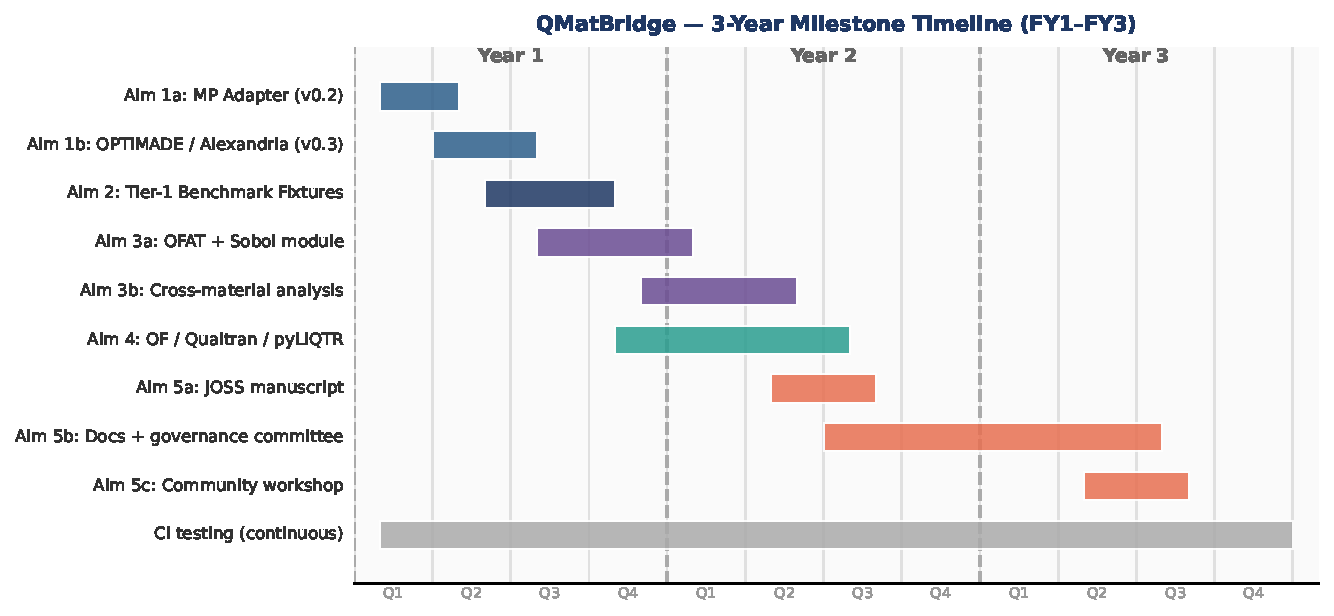
\includegraphics[width=\linewidth]{fig_gantt.pdf}
\caption{Three-year milestone timeline (FY1--FY3, quarter resolution).
Color encodes aim: Aim 1 = blue, Aim 2 = navy, Aim 3 = purple,
Aim 4 = teal, Aim 5 = orange, CI/testing = gray.
Dashed vertical lines mark federal fiscal year boundaries.}
\label{fig:gantt}
\end{figure}

%% ============================================================
\section{Conclusion}

QMatBridge addresses a foundational infrastructure gap in the quantum
simulation of materials: the absence of a shared, provenance-rich,
machine-readable data standard connecting classical DFT databases to
fault-tolerant quantum algorithms.
Preliminary results demonstrate technical feasibility across schema
design, sensitivity analysis, and multi-objective benchmark selection.
The proposed work will complete the adapter and exporter layers,
build the Tier-1 benchmark fixture set, and establish the community
governance structures required for long-term sustainability.
The outcome will be a community-maintained data infrastructure that
enables reproducible, citable quantum simulation benchmarks --- a
prerequisite for the field to progress from isolated resource estimates
to a coherent, cross-group understanding of where quantum advantage for
materials simulation can realistically be achieved.

%% ============================================================
\newpage
\bibliographystyle{unsrtnat}
\bibliography{references}

\end{document}
